\section{The reference box: what one line actually measures}
\label{sec:msres}

\noindent\emph{Status: draft -- every number below is read from one record, the \texttt{npml}${}=10$ audit run
dumped to \texttt{.scratch/study\_dump.txt}. Nothing is re-derived from an earlier revision and nothing is
imported from a second geometry. Where that record carries two values for one quantity, both are printed and the
difference is discussed rather than averaged away.}

\subsection{The reference box}
\label{sec:msres-box}

Everything in this section is one geometry, named once here so that no later number has to be qualified by which
box it belongs to. The \emph{reference box} is a microstrip of strip width $w = 3.20$ mm on a substrate of
thickness $h = 1.60$ mm, so $w/h = 2.000$, with $\eps_r = 4.4$, on a mesh of $66\times52\times26$ cells of
$0.400$ mm covering $26.40\times20.80\times10.40$ mm. The matched layer is ten cells thick on every face. The run
is $2400$ leapfrog steps, of which the last $1800$ are transformed: the first $600$ are warm-up and are excluded
from every average, fit and accounting below. The drive is a lumped gap source at $5.8278$ GHz, which is where
the requested $6.0000$ GHz lands after being snapped to a discrete Fourier bin, and the run takes $31.79$ s.
Nine station planes record the complex line voltage from $x = 10.40$ mm to $x = 20.00$ mm, a span of $9.60$ mm;
the first of them is the port plane and the reference plane of the scattering parameters. The far plane of the
line sits $21.6$ mm from the port plane, and the difference between the two lengths is large enough that it is
stated again wherever it is used: $9.60$ mm is measured, $21.6$ mm is extrapolated.

That the record is a steady state and not a transient is checked rather than assumed. Fitting $\beta$ over the
two halves of the transformed record gives $231.973$ rad/m over the first half and $231.798$ rad/m over the
second, $0.076$ per cent apart against the $1.0$ per cent this study allows, so any window of it is a fair
sample of the steady state and the warm-up exclusion is doing its job.

\subsection{Three impedances on one record}
\label{sec:msres-z0}

Table~\ref{tab:ms-z0} collects every impedance the record yields. The Hammerstad--Jensen figure of $48.686\ \Ohm$
is printed beside each of them as a reference, not as a target: it is a closed form for a static problem, and the
comparison is a diagnostic of the order of the answer, which Section~\ref{sec:ms-quasithem} argues is all such a
comparison can be.

\begin{table}[H]
  \centering
  \caption{Every impedance the reference box yields. The last column compares against the closed form
  $48.686\ \Ohm$ evaluated at this geometry; it is a diagnostic, not a tolerance. The modulus rows are printed so
  that the inflation of Section~\ref{sec:ms-z0} can be seen happening, not because a modulus is a characteristic
  impedance.}
  \label{tab:ms-z0}
  \small
  \begin{tabular}{@{}>{\raggedright\arraybackslash}p{0.42\textwidth}rr@{}}
    \toprule
    Quantity & Value & Ratio to $48.686\ \Ohm$ \\
    \midrule
    Port plane, real part                                  & $50.952\ \Ohm$              & $1.0466$ \\
    Port plane, modulus                                    & $53.144\ \Ohm$              & $1.0916$ \\
    Port plane, phase (excess, trace-current reference)    & $16.512^\circ$              & --- \\
    Station fit, real part (decay held fixed)              & $51.1768\ \Ohm$             & $1.0512$ \\
    Station fit, modulus                                   & $51.3099\ \Ohm$             & $1.0539$ \\
    Station fit, phase (two-wave, forward current)         & $4.1268^\circ$              & --- \\
    Station fit, uncertainty (stat.)                       & $0.1128\ \Ohm$             & --- \\
    Station fit, uncertainty (from $\beta$)                & $0.0002\ \Ohm$             & --- \\
    Station fit, real part, decay left free                & $51.1791 \pm 0.0735\ \Ohm$  & $1.0512$ (${+}5.121$ per cent) \\
    Power--current, mean over stations                     & $51.1648\ \Ohm$             & --- \\
    Power--current, spread over $9$ stations               & $1.0572\ \Ohm$              & --- \\
    Power--current ratio, mean                             & $0.999766$                  & --- \\
    Power--current ratio, worst station ($20.00$ mm)       & $0.988790$                  & --- \\
    Power--current ratio at the port plane                 & $1.000000$ (identity)       & --- \\
    Mode purity, $|\gamma_I + \gamma_V|$                   & $6.808\times10^{-3}$        & --- \\
    \bottomrule
  \end{tabular}
\end{table}

The first two rows are the trap the theory section warns about, and this record walks into it. The port-plane
impedance is $50.952 + 15.105j\ \Ohm$: a real part, a reactance, and a modulus of $53.144\ \Ohm$ that is neither.
The phase is the lumped source's own reactance, and the modulus is the real part inflated by
$1/\cos 16.512^\circ = 1.0430$ -- exactly the factorisation of \eqref{eq:ms-zplane}, with nothing left over. So
the two comparisons in the table are not two measurements of one quantity: the real part is $4.66$ per cent from
the closed form and the modulus is $9.16$ per cent from it, and the whole of the difference between those two
figures is the source's reactance. A paper that printed $53.144\ \Ohm$ as ``the measured $Z_0$'' would be
reporting its own generator.

The station fit is the measurement, and there the same inflation is visible but ten times smaller: a residual
phase of $4.1268^\circ$ turns a real part of $51.1768\ \Ohm$ into a modulus of $51.3099\ \Ohm$, a factor of
$1.0026$. At the size of the discrepancy being discussed -- $5.1$ per cent from the closed form -- the choice
between those two numbers is immaterial, which is why Table~\ref{tab:ms-z0} gives both and neither is promoted.
Its uncertainty is $0.1128\ \Ohm$ statistical, with $0.0002\ \Ohm$ contributed by the uncertainty in $\beta$: the
impedance is an amplitude ratio and barely cares about the phase constant. Letting the decay float moves the real
part to $51.1791 \pm 0.0735\ \Ohm$, a shift of $+0.0023\ \Ohm$ that is three times inside its own error bar, so
the lossless and lossy fits do not disagree about $Z_0$; what the free decay costs is the error budget, which now
carries the $\alpha$ term squared in it.

The power--current estimator is the one that is not independent, and the table says so twice. At the port plane
its ratio is $1.000000$ because it is $1$ by construction: on that plane $Z_0$ \emph{is} $V/I$, so the two
phasors are one number and the row can differ from unity only by round-off. It is an identity check, not a
measurement. The stations row is the measurement, and it holds to $0.999766$ on average with a spread of
$1.0572\ \Ohm$ and a worst station of $0.988790$ at $20.00$ mm. That spread is not free-floating error: the
passive reflection this box carries, $|\gamma| = 0.0060$, can move a power ratio by at most $2.4$ per cent, and
the observed spread of $2.07\times10^{-2}$ sits inside that bound. The spread is the standing wave seen a second
time, not a second mechanism. Mode purity, $|\gamma_I + \gamma_V| = 6.808\times10^{-3}$ against $0$ for a pure
mode, says the same thing from the other side: the record is one mode plus a residue at the $0.7$ per cent level,
which is the number the ``not quite one mode'' remarks elsewhere in this report should be read against.

\subsection{Four rates for one attenuation}
\label{sec:msres-alpha}

Table~\ref{tab:ms-alpha} is the estimator problem of Section~\ref{sec:ms-estimators} made numeric on one record.
Two of the five estimators listed there collapse into one row here: the endpoint ratio and the model-free end
ratio are the same arithmetic, $|V_N|/|V_1|$ of the raw station amplitudes, so a record that does not subtract a
backward wave first cannot distinguish them and this one does not. The forward-subtracted variant is not reported
separately by this record. What is left is four rates, and they span a factor $1.86$.

\begin{table}[H]
  \centering
  \caption{Four estimates of one attenuation on the reference box, with the $|S_{21}|$ each implies. The two
  right-hand columns apply $\exp(-\alpha L)$ over, respectively, the measured station span and the extrapolation
  to the far plane; the last row is a bound over the short span only and is not extrapolated, because it is
  already an upper bound (Section~\ref{sec:ms-accounting}).}
  \label{tab:ms-alpha}
  \begin{tabular}{@{}lrrr@{}}
    \toprule
    Estimator & $\alpha$ [dB/mm] & $|S_{21}|$, $9.60$ mm & $|S_{21}|$, $21.6$ mm \\
    \midrule
    One-wave joint fit            & $0.02145 \pm 0.00117$ & $0.9766$ & $0.948$ \\
    Two-wave joint fit            & $0.02164 \pm 0.00067$ & $0.9764$ & $0.948$ \\
    Direct station-plane ratio    & $0.01183$             & $0.9870$ & $0.971$ \\
    Lateral-wall accounting       & $0.01160$             & $0.9873$ & $0.972$ \\
    Same work charged to the span & $0.03311$ (bound)     & $0.9641$ & not extrapolated \\
    \bottomrule
  \end{tabular}
\end{table}

The two fits agree with each other and disagree with everything else. They are almost orthogonal in their own
parameter space -- $\rho(\alpha,\beta) = -0.0000$ from the $2\times2$ block of $s^2(D^{\mathsf T}D)^{-1}$ on those
two parameters, over $18$ measurements -- so the decay costs the phase constant almost nothing to measure, and the
agreement between the one-wave and two-wave fits is not the agreement of two independent estimators: both are
fitting the same exponential to the same ripple. The direct ratio and the accounting rate are the two that share
no machinery with them, and those two agree to $1.9$ per cent. That pattern is the finding of the next subsection.

On the phase constant the record is consistent with itself and with nothing else. The one-wave fit gives
$\beta = 231.886 \pm 0.134$ rad/m and the two-wave fit $232.419 \pm 0.078$ rad/m, while a summary line of the same
record quotes $232.400$ rad/m with no uncertainty -- the value with an uncertainty attached is the one quoted
here. The closed form gives $223.353$ rad/m, so the fit is $3.82$ per cent above it ($4.06$ per cent for the
two-wave value), and $\eps_{\mathrm{eff}}$ follows: $3.60431$ measured against $3.34394$ from the closed form, a
difference of $7.8$ per cent. These comparisons are labelled diagnostic in the record itself and they stay
labelled that way here. The closed form is quasi-static; the measurement is not. A $3.8$ per cent gap between
them says the quasi-TEM model is the wrong problem at this $w/h$, and says nothing about whether the solver is
right.

The extrapolation column deserves one sentence of warning. Nothing in this record measures $21.6$ mm of line; the
longest distance any two of its numbers span is $9.60$ mm. Applying $\exp(-\alpha L)$ over $21.6$ mm assumes the
decay is exponential over a length $2.25$ times the one that was fitted, and the reason to print it anyway is that
the acceptance criterion below is stated on the longer line, so the reader is entitled to see what each estimator
would say there. It is the exercise that shows $0.948$ and $0.972$ to be the two ends of one instrument's range.

\subsection{Where the power went}
\label{sec:msres-accounting}

The accounting of Section~\ref{sec:ms-accounting} is available on this record because the audit kept the work the
matched layer removed, split by wall family, over exactly the $1800$ settled steps the transform saw.
Table~\ref{tab:ms-acct} is that split. In the steady state every joule injected is absorbed, so the total is the
injected energy and each share is a share of the injected power.

\begin{table}[H]
  \centering
  \caption{Work removed by the matched layer over the $1800$ accounted steps, by wall family, with the rate
  \eqref{eq:ms-accounting} assigns to each. Only the lateral family runs along the line, so only it converts into
  a per-unit-length rate; the end walls are the intended absorbers and their work belongs to no length of line.}
  \label{tab:ms-acct}
  \small
  \begin{tabular}{@{}lrrrr@{}}
    \toprule
    Wall family & Share & Work [J] & Length [mm] & $\alpha$ [Np/m] \\
    \midrule
    Lateral ($y_{\min}$, $y_{\max}$, top) & $7.054$ per cent & $1.976361\times10^{-7}$ & $26.40$ & $1.3360$ \\
    End ($x_{\min}$, $x_{\max}$)          & $92.946$ per cent & $2.604064\times10^{-6}$ & --- & --- \\
    Total                                 & $100$ per cent & $2.801700\times10^{-6}$ & --- & --- \\
    \bottomrule
  \end{tabular}
\end{table}

The lateral rate is $1.3360$ Np/m, which is $0.01160$ dB/mm. Set against it, the direct station-plane ratio is
$0.01183$ dB/mm -- $1.9$ per cent away -- and the one-wave fit is $0.02145$ dB/mm, $1.84$ times the absorbed rate
($1.85$ times for the two-wave value). That ordering is the result of this section and it is stated as a finding
rather than as a discrepancy: \emph{two model-free measurements agree with each other and the fit is the outlier},
so the attenuation this box exhibits is a lateral boundary sink of $0.0116$ dB/mm and not conductor loss -- which
it could not be in any case, since the solver contains no ohmic term. What that sink physically is, the
accounting does not say: Section~\ref{sec:msres-verdict} names the two candidates it leaves, and the clearance
test it carries separates them. Over the $21.6$ mm of the line the sink costs $0.25$ dB, and $|S_{21}| = 0.972$;
that magnitude belongs to this box rather than to the line, as the clearance test in
Section~\ref{par:msres-mechanism} shows.

The last row of Table~\ref{tab:ms-alpha} is the same work charged the other way, and it is printed to keep the
arithmetic honest. The lateral walls run $26.40$ mm of line; charging all of their work to the $9.60$ mm station
span assumes every joule they removed was removed beside the stations, which overstates the rate by the ratio of
the lengths, $2.75$, and lands on $0.0331$ dB/mm and $|S_{21}| = 0.9641$. That number is an upper bound and is
usable as nothing else; it is in the table because it is the number a careless reading of the accounting produces,
and because a reader who recomputes it from the raw work should find the same $0.9641$ and then the same
explanation.

\subsection{The acceptance outcome}
\label{sec:msres-verdict}

Section~\ref{sec:ms-criterion} asks three things of a run, and the reference box can be graded against all three
without choosing an estimator by taste. Two of them are met outright; the third is met by identifying the
mechanism, and the two qualifications that carries are stated where they arise.

First, $|S_{21}|$ must be consistent with a lossless \emph{material} model within the stated uncertainty of the
measurement. The direct ratio, $|S_{21}| = 0.987008$, is $1.299$ per cent below unity. The span the estimators
produce over the
same $9.60$ mm runs from $0.9764$ to $0.9873$, so $0.987008$ sits at the lossless end of that span, and $1.3$ per
cent is inside the $2.5$ to $3$ per cent this record can resolve. This requirement is met.

Second, the attenuation that remains must be attributed with its magnitude accounted for. The measured rate is
$0.01183$ dB/mm; the lateral-wall accounting, which counts joules and never looks at the amplitude record,
predicts $0.01160$ dB/mm. The two agree to $1.9$ per cent, which is an attribution that pays for the whole of the
effect rather than a name attached to a residual. This requirement is met.

Third, the mechanism must be identified by name and by the part of the box responsible for it. The part is
settled: the matched layer on $y_{\min}$, $y_{\max}$ and the top face removed $7.054$ per cent of the injected
power in the settled window while the end walls took the remaining $92.946$, so the sink sits on the lateral and
lid faces and nowhere else. Two candidates were stated for the mechanism itself: absorption of a slowly decaying
lateral tail by the matched layer, and a propagating lateral component of the box-loaded mode that a wider box
would not cure. The clearance test below discriminates between them and selects the first. A second argument
selects the same one without using the clearance at all: the matched layer sits $4.80$ mm above the strip, which
is $0.95$ of a lateral decay length, so the region above the strip is below cutoff vertically and there is no
half-space in which a grounded-slab $\mathrm{TM}_0$ wave could exist, whatever the lateral wall does.
\label{par:msres-mechanism}

Both tests that follow use the \texttt{Board} path: a board object carrying the stack-up, the trace and the port
is converted from millimetre drawing units to SI metres and run through the same solver, so the geometry can be
widened without touching the mesh. Both tests were pre-registered: the predicted bands were written down before
the solve. The substrate-thickness test did not discriminate. The audited lateral wall work is $0.011604$ dB/mm
at $h = 1.60$ mm and $0.004322$ dB/mm at $h = 0.80$ mm with $w/h$ held at $2.000$, a ratio of $0.372$, that is
$h$ to the $1.425$. Both candidates predict a fall with thickness, and $0.372$ lies between the $h$ and
$h$-squared keys, so it separates neither. Only the audited wall work and the absorbed-work totals carry that
scaling; the fitted attenuation and the station ratio are unusable at the thinner substrate, and that estimator
disagreement is itself the reason the audit exists. What the test did establish is that the sink is not a
material attenuation: it scales with the geometry as a boundary term, and it falls per unit stored power faster
than the stored power falls.

The clearance test is the one that discriminates. Widening the board from $20.80$ mm to $28.80$ mm, which puts
$8.8$ mm of clean dielectric either side of the strip instead of $4.8$ mm and changes nothing else, took the
audited lateral work from $1.33601$ Np/m to $0.60085$ Np/m, a ratio of $0.450$. The work on the edge cells where
the walls meet fell to $0.471$ of its value and the work on the wall face cells to $0.435$, so the fall is a
redistribution neither between field families nor between wall families; the end-wall work moved by $4.4$ per
cent, and $\beta$ moved from $231.89$ rad/m to $232.14$ rad/m while $\varepsilon_{\mathrm{eff}}$ moved from
$3.6043$ to $3.6123$, so the mode itself did not change. The pre-registered band for a propagating lateral
component was $0.75$ to $1.05$ and is excluded by the audited work, while the band for a decaying tail was
$0.21$ to $0.50$ and contains the result at its upper edge. The ratio therefore selects: $0.450$ is the fall a
decaying tail predicts and not the fall a laterally propagating mode predicts, which would hold near unity as the
wall moves, and the lid argument rules out the grounded-slab alternative independently. The sink is the decaying
tail of the discretised mode absorbed at the lateral boundary, and the strip is not radiating that power. The
margin is not generous -- $0.450$ sits at the upper edge of the band it satisfies, $1.11$ times inside it -- and
what makes the reading firm is the second band rather than the first: the same number is $1.67$ times below the
nearer edge of the band it excludes.

The magnitude of that sink is set by the clearance, so $0.011604$ dB/mm is a property of this box and not of the
line, and the audited sink in the wide box is $0.00522$ dB/mm for the same strip. The total
attenuation falls less than the sink does, and that difference is visible with a single estimator carried across
the two boxes: the audited lateral work falls to $0.450$ of its value, while the plain station-to-station rate
over the same $9.60$ mm falls from $1.36215$ Np/m to $0.91350$ Np/m, a ratio of $0.671$, and the fitted
attenuation falls to $0.590$ of its reference-box value. Only the audited ratio selects: $0.671$ lies in the
$0.50$ to $0.75$ gap between the two registered bands, where neither reading is favoured, so it is reported and
not used. Every estimator falls when the box is widened and none
stays put, so the decay measured in the reference box is not an attenuation set by the line: a quantity fixed by
the line would not move when the wall moves. What remains open is how the between-station decay divides. In the
reference box the audited lateral work reproduces the endpoint rate to within $2$ per cent, a factor of $1.02$,
so there the sink is the whole of the decay within the accuracy of that comparison. In the wide box the lateral
bin accounts for only two thirds of it, a factor of $1.52$, which leaves $0.31$ Np/m of the between-station
decay unaccounted for by that bin. Two readings survive one run: either the endpoint rate carries an error of
order $0.2$ Np/m at a rate near $0.9$ Np/m, or there is a component of the decay that does not depend on the
clearance and that the lateral bin does not capture, and nothing in this record decides between them. What a
closed box cannot do is separate layer absorption from radiation in general: a wider box cures both, so the test
above separates the two candidates it was registered against and no further pair, and a demonstration that the
strip radiates nothing at all would need an open boundary or a clearance convergence study.

So the criterion is met on the reference box in the form the record can grade it in: $|S_{21}|$ is consistent
with a lossless material model, the shortfall is attributed to a sink whose magnitude the energy balance pays for
to $1.9$ per cent, and the sink is located in the box. The mechanism requirement is met in the sense the
criterion asks for: the sink is a boundary artefact, the decaying tail of the discretised mode absorbed at the
lateral layer, and not a power the strip radiates. Two qualifications travel with that. The first is the
$0.31$ Np/m of wide-box between-station decay that the lateral bin does not account for, so the sink is
identified while the decay of this geometry is not yet fully binned. The second is the generality of the claim:
a closed box cannot separate layer absorption from radiation, so what is established is the sink of this box and
not the radiation of the strip in every box. A third qualification
is that it is met by the estimator with no free parameter. The one-wave fit reads $|S_{21}| = 0.976570$, $2.343$
per cent below unity and $1.84$ times the absorbed rate, which fails the first requirement on its own. The criterion is
therefore not something a run passes; it is something a particular \emph{measurement} passes, and the report says
which.

The reflection result belongs beside it. $|S_{11}| = 0.00597$, which is $-44.48$ dB, at both the measured plane at
$x = 10.40$ mm and the port plane after de-embedding with $d = 5.60$ mm; $\beta$ is real, so the move changes the
phase and nothing else. As a mismatch that is VSWR $1.0120 : 1$, from $(1+|\gamma|)/(1-|\gamma|)$ with
$|\gamma| = 0.00597$. The goal of $-20$ dB is met with $24$ dB to spare.

One number in this record is not reconciled, and it is left that way rather than smoothed. The same dump carries
$|\gamma| = 0.00628$ in its summary line and $|S_{11}| = 0.00597$ in the rows that refer to the planes: $5.2$ per
cent apart for what should be one reflection coefficient. The summary figure is the two-wave fit's $\gamma$, the
one quoted in the mid-plane figure's caption and used for the ripple bound of Section~\ref{sec:ms-criterion}; the
$0.00597$ is the reflection actually measured at the reference plane, and it is the one quoted as $|S_{11}|$
wherever a scattering parameter is meant. Both are consistent with ``about $-44$ dB'', the power-ratio bound
above is insensitive to which is used, and no downstream number changes. But the $5.2$ per cent itself has no
account in this record, so it is flagged as unreconciled rather than explained.

\subsection{Two kinds of rate, and why they are not compared}
\label{sec:msres-estimators}

A fitted attenuation and an audited one are not two measurements of one quantity. A fit is a property of the
window: its slope depends on which stations lie inside the window, on whether a backward wave is modelled, and on
how much of a ripple period the window covers. The audited rate is a property of the geometry: it commits in
advance to a power budget, divides the work a wall family removed by the length of wall that removed it, and
never looks at an amplitude. Both are legitimate and neither refines the other; a discrepancy measures the
distance between two estimators, and no conclusion about the box follows until both are computed the same way.

The reference box shows that distance with no change of geometry. Its own record, over its own $9.60$ mm, gives a
fitted rate of $0.02145$ dB/mm, which is $2.47$ Np/m, against an audited $1.33601$ Np/m: a factor of $1.84$ on
one geometry and one window, so the factor is estimator difference and says nothing about clearance or mechanism.
This work once read it the other way, as a fit that was right and an audit that was short; that took a ratio
between estimators for a discrepancy against a truth, and it was wrong. The $1.600$ Np/m an earlier sweep reports
for fitted values over $14.4$ mm is comparable with neither, its window and its geometry both differing.

Comparisons that do hold are inside one estimator across boxes: audited lateral work falls to $0.450$, the fitted
attenuation to $0.590$, the endpoint ratio to $0.671$, and only the first of the three selects. A fitted
attenuation here is therefore a property of the window and the estimator and not of the line, which is why the
criterion of Section~\ref{sec:ms-criterion} rests on audited work and the station ratio, not on a fit.

\subsection{The record in pictures}
\label{sec:msres-figs}

\begin{figure}[H]
  \centering
  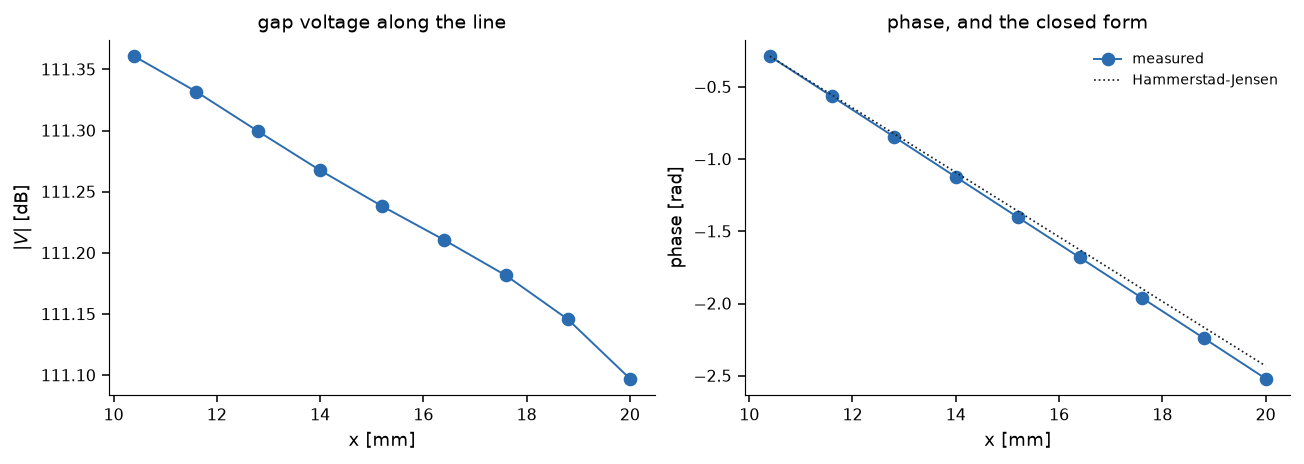
\includegraphics[width=0.92\textwidth]{../figures/ms-line-phasors.png}
  \caption{The record the estimators are fitted to. Left: $|V|$ in decibels at the nine station planes against
  $x$ in millimetres. Right: the unwrapped phase in radians against $x$, with the closed-form
  Hammerstad--Jensen ramp dotted beside it -- the closed form is a straight line of the slope the model predicts,
  not a fit to the points. The envelope falls by $3.0$ per cent across the span while each half fit is good to
  $1.4\times10^{-3}$; the ripple riding on that fall is the standing wave of
  Section~\ref{sec:msres-verdict}, and it is why a single exponential through these points absorbs a bias.}
  \label{fig:ms-phasors}
\end{figure}

\begin{figure}[H]
  \centering
  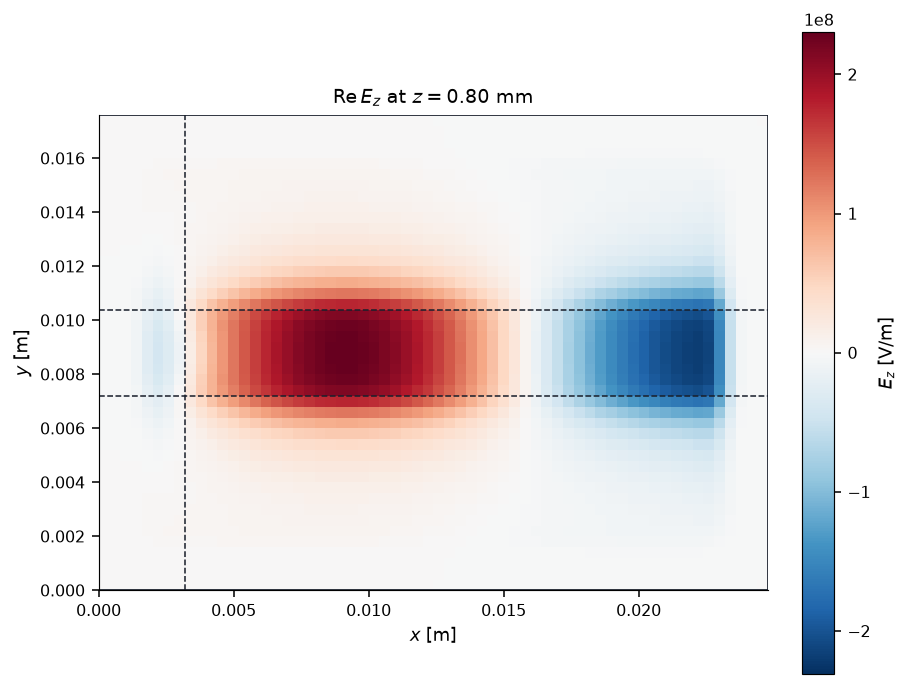
\includegraphics[width=0.62\textwidth]{../figures/ms-midplane-ez.png}
  \caption{Real part of the $5.8278$ GHz phasor of $E_z$ in volts per metre, on the node layer halfway up the
  $1.60$ mm substrate ($z = 0.80$ mm at the reference box's cell size), taken as the mean of the two cells that
  straddle that layer. The phasors are complex and a colour map is not, so the real part is what is drawn: this is
  the field at the phase the accumulated record starts on, not an amplitude. Dashed: the port plane and the two
  strip edges. The fringes along the line are the forward wave beating with the backward one, whose coefficient
  this record puts at $|\gamma| = 0.0063$; an amplitude plot would show a monotone taper and none of them.}
  \label{fig:ms-midplane}
\end{figure}

The two figures are the record itself rather than a summary of it, and they are worth reading against the tables
in one respect only: the phase panel's slope and the magnitude panel's fall are the two quantities
Table~\ref{tab:ms-alpha} disagrees with itself about, and both are visible by eye. What they do not show, and
what the accounting table does, is where the power went -- a picture of the line cannot distinguish a mode that
decayed in place from one that lost power to the lateral walls, because both look like a falling envelope on the
axis the stations sit on.
